% Title: glps_renderer figure
% Creator: GL2PS 1.3.8, (C) 1999-2012 C. Geuzaine
% For: Octave
% CreationDate: Tue Dec 15 01:59:43 2015
\setlength{\unitlength}{1pt}
\begin{picture}(0,0)
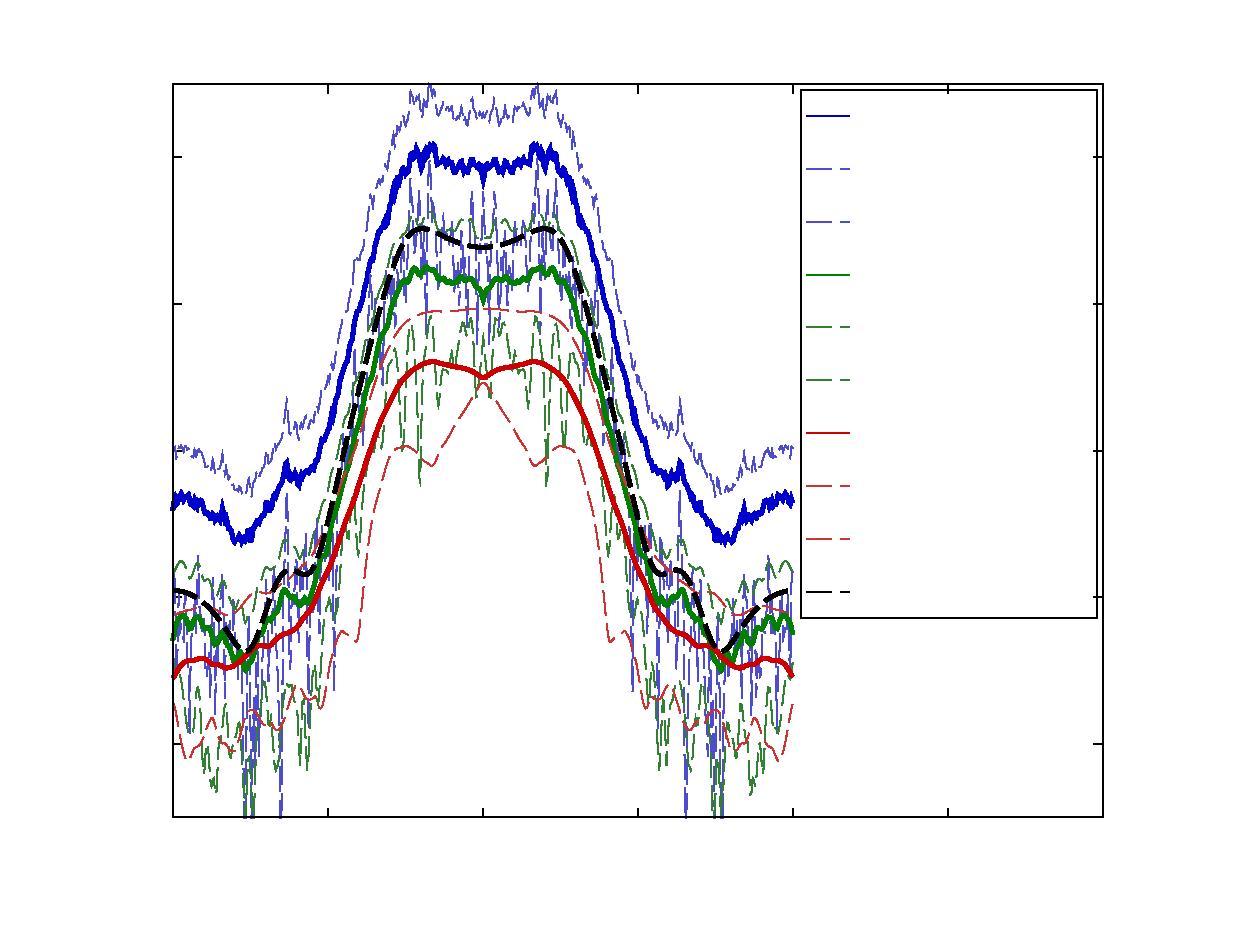
\includegraphics{Imagenes/no_param_2c-inc}
\end{picture}%
\begin{picture}(576,432)(0,0)
\fontsize{10}{0}
\selectfont\put(74.88,42.5189){\makebox(0,0)[t]{\textcolor[rgb]{0,0,0}{{0}}}}
\fontsize{10}{0}
\selectfont\put(149.28,42.5189){\makebox(0,0)[t]{\textcolor[rgb]{0,0,0}{{0.5}}}}
\fontsize{10}{0}
\selectfont\put(223.68,42.5189){\makebox(0,0)[t]{\textcolor[rgb]{0,0,0}{{1}}}}
\fontsize{10}{0}
\selectfont\put(298.08,42.5189){\makebox(0,0)[t]{\textcolor[rgb]{0,0,0}{{1.5}}}}
\fontsize{10}{0}
\selectfont\put(372.48,42.5189){\makebox(0,0)[t]{\textcolor[rgb]{0,0,0}{{2}}}}
\fontsize{10}{0}
\selectfont\put(446.88,42.5189){\makebox(0,0)[t]{\textcolor[rgb]{0,0,0}{{2.5}}}}
\fontsize{10}{0}
\selectfont\put(521.28,42.5189){\makebox(0,0)[t]{\textcolor[rgb]{0,0,0}{{3}}}}
\fontsize{10}{0}
\selectfont\put(69.8755,82.728){\makebox(0,0)[r]{\textcolor[rgb]{0,0,0}{{-40}}}}
\fontsize{10}{0}
\selectfont\put(69.8755,153.144){\makebox(0,0)[r]{\textcolor[rgb]{0,0,0}{{-20}}}}
\fontsize{10}{0}
\selectfont\put(69.8755,223.56){\makebox(0,0)[r]{\textcolor[rgb]{0,0,0}{{0}}}}
\fontsize{10}{0}
\selectfont\put(69.8755,293.976){\makebox(0,0)[r]{\textcolor[rgb]{0,0,0}{{20}}}}
\fontsize{10}{0}
\selectfont\put(69.8755,364.392){\makebox(0,0)[r]{\textcolor[rgb]{0,0,0}{{40}}}}
\fontsize{10}{0}
\selectfont\put(298.08,29.5189){\makebox(0,0)[t]{\textcolor[rgb]{0,0,0}{{\omega * \pi}}}}
\fontsize{10}{0}
\selectfont\put(49.8755,223.56){\rotatebox{90}{\makebox(0,0)[b]{\textcolor[rgb]{0,0,0}{{PSD [dB]}}}}}
\fontsize{10}{0}
\selectfont\put(298.08,409.6){\makebox(0,0)[b]{\textcolor[rgb]{0,0,0}{{Periodograma promedio y, \phi_y, N = 256}}}}
\fontsize{10}{0}
\selectfont\put(402.654,384.173){\makebox(0,0)[l]{\textcolor[rgb]{0,0,0}{{M = N, E[\phi_y]}}}}
\fontsize{10}{0}
\selectfont\put(402.654,358.803){\makebox(0,0)[l]{\textcolor[rgb]{0,0,0}{{M = N, E[\phi_y] + \sigma_{\phi_y}}}}}
\fontsize{10}{0}
\selectfont\put(402.654,333.433){\makebox(0,0)[l]{\textcolor[rgb]{0,0,0}{{M = N, E[\phi_y] - \sigma_{\phi_y}}}}}
\fontsize{10}{0}
\selectfont\put(402.654,308.063){\makebox(0,0)[l]{\textcolor[rgb]{0,0,0}{{M = N/4, E[\phi_y]}}}}
\fontsize{10}{0}
\selectfont\put(402.654,282.692){\makebox(0,0)[l]{\textcolor[rgb]{0,0,0}{{M = N/4, E[\phi_y] + \sigma_{\phi_y}}}}}
\fontsize{10}{0}
\selectfont\put(402.654,257.322){\makebox(0,0)[l]{\textcolor[rgb]{0,0,0}{{M = N/4, E[\phi_y] - \sigma_{\phi_y}}}}}
\fontsize{10}{0}
\selectfont\put(402.654,231.952){\makebox(0,0)[l]{\textcolor[rgb]{0,0,0}{{M = N/16, E[\phi_y]}}}}
\fontsize{10}{0}
\selectfont\put(402.654,206.582){\makebox(0,0)[l]{\textcolor[rgb]{0,0,0}{{M = N/16, E[\phi_y] + \sigma_{\phi_y}}}}}
\fontsize{10}{0}
\selectfont\put(402.654,181.211){\makebox(0,0)[l]{\textcolor[rgb]{0,0,0}{{M = N/16, E[\phi_y] - \sigma_{\phi_y}}}}}
\fontsize{10}{0}
\selectfont\put(402.654,155.841){\makebox(0,0)[l]{\textcolor[rgb]{0,0,0}{{\phi_y Teórico}}}}
\end{picture}
